\documentclass[12pt, twoside]{article}
\usepackage[letterpaper, margin=1in, headsep=0.5in]{geometry}
\usepackage[english]{babel}
\usepackage[utf8]{inputenc}
\usepackage{amsmath}
\usepackage{amsfonts}
\usepackage{amssymb}
\usepackage{tikz}
\usetikzlibrary{quotes, angles}
\usepackage{graphicx}
\usepackage{enumitem}
\usepackage{multicol}

\newif\ifmeta
\metatrue %print standards and topics tags

\title{IB Math Applications and Interpretations}
\author{Chris Huson}
\date{March 2022}

\usepackage{fancyhdr}
\pagestyle{fancy}
\fancyhf{}
\renewcommand{\headrulewidth}{0pt} % disable the underline of the header
\raggedbottom

\fancyhead[LE]{\thepage}
\fancyhead[RO]{\thepage \\ Name: \hspace{4cm} \,\\}
\fancyhead[LO]{BECA / IB Math 6 Geometry \\* 14 April 2022}

\begin{document}
\subsubsection*{6.13 Test Geometry \hfill HSG.SRT.D.11}
\emph{Find exact values or round decimal approximations to three significant figures.}
\begin{enumerate}
\item As shown, right $\triangle ABC$ has $AC=8, BC=15, AB=17$, $m\angle C=90^\circ$. \\[0.25cm] 
Express each trigonometric ratio as a fraction.
  \begin{multicols}{2}
    \begin{enumerate}[itemsep=0.2cm]
      \item $\sin A =$
      \item $\cos A =$
      \item $\tan A =$
      \item Find $m\angle A$.
    \end{enumerate}
    \begin{center}
      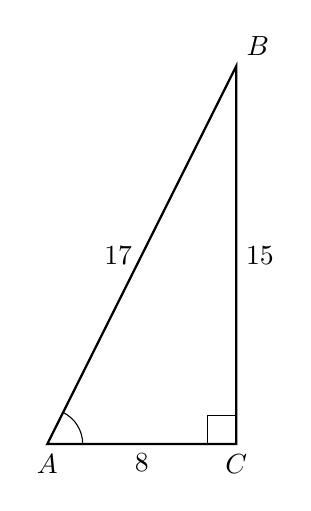
\begin{tikzpicture}[scale=0.6]
        \draw [thick](0,0) node[below]{$A$}--
        (4,0) node[below]{$C$}--
        (4,8) node[above right]{$B$}--cycle;
        \node at (2,0)[below]{$8$};
        \node at (4,4)[right]{$15$};
        \node at (2,4)[left]{$17$};
        \draw (4,0)++(-0.6,0)--++(0,0.6)--+(0.6,0);
        \draw (0.75,0) arc [start angle=0, end angle=63, radius=0.75];
      \end{tikzpicture}
    \end{center}
  \end{multicols} \vspace{1cm}

\item Right triangle $\triangle ABC$ is shown with measures as marked.\vspace{0.25cm}
\begin{multicols}{2}
  \begin{enumerate}[itemsep=0.5cm]
    \item Write down $\sin A$.
    \item Find the length of side $AC$.\vspace{1.5cm}
    \item Find the angle measure of $\angle A$.
    \vspace{1cm}
  \end{enumerate}
\begin{flushright}
        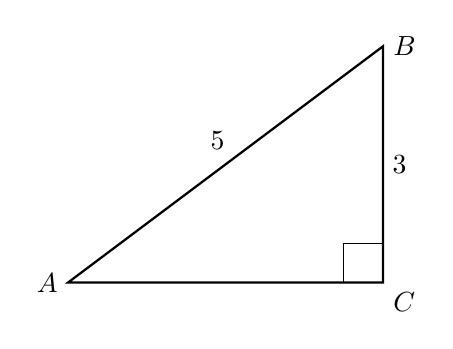
\begin{tikzpicture}[scale=1]
        \draw [thick]
        (0,0)node[left]{$A$}--
        (4,0)node[below right]{$C$}--
        (4,3)node[right]{$B$}--cycle;
        \draw (4,0)++(-0.5,0)--++(0,0.5)--+(0.5,0);
        \node at (4,1.5)[right]{$3$};
        \node at (1.9,1.8){$5$};
        %\node at (4,2.7)[right]{$8$};
        %\node at (1.8,2.6)[above]{$10$};
      \end{tikzpicture}
\end{flushright}
\end{multicols} \vspace{1.5cm}

\item Right triangle $ABC$ is shown with $AB=55$, $m\angle A=41^\circ$. Find the value of $BC=x$.
  \begin{flushright}
    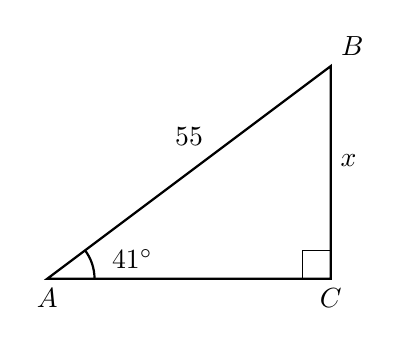
\begin{tikzpicture}[scale=0.6]
      \draw [thick](0,0)node[below]{$A$}--
      (6,0)node[below]{$C$}--
      (6,4.5)node[above right]{$B$}--cycle;
      \draw (6,0)++(-0.6,0)--++(0,0.6)--+(0.6,0);
      \node at (3,3){$55$};
      \node at (6,2.5)[right]{$x$};
      \draw [thick, -] (1,0) arc [start angle=0, end angle=37, radius=1];
      \node at (1.8,0)[above]{$41^\circ$};
    \end{tikzpicture}
  \end{flushright}

\newpage
\subsubsection*{Given formulas}
Sine rule: $\displaystyle \frac{a}{\sin A} = \frac{b}{\sin B} = \frac{c}{\sin C}$ \\[0.5cm]
Cosine rule: $c^2 = a^2+b^2- 2ab \cos C$, \,
$\displaystyle \cos C=\frac{a^2+b^2-c^2}{2ab}$\\[0.5cm]
Area of a triangle: $\displaystyle A=\frac{1}{2}ab \sin C$ \\[0.5cm]

\item Find the area of the given triangle.
\begin{flushright}
  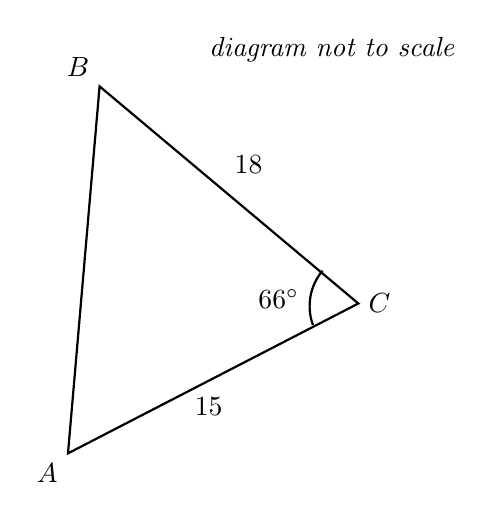
\begin{tikzpicture}[scale=0.7]
    \draw [thick](0:4)node[right]{$C$}--
    (100:4)node[above left]{$B$}--
    (-115:3)node[below left]{$A$}--cycle;
    \node at (55:3.5)[below]{$18$};
    \node at (-50:2)[below]{$15$};
    \draw [thick, -] (-7:3.2) arc [start angle=200, end angle=140, radius=1];
    \node at (1.5:3.1)[left]{$66^\circ$};
    \node at (50:5.5)[above]{\emph{diagram not to scale}};
  \end{tikzpicture}
\end{flushright}

\item The following diagram shows triangle $ABC$, with $A\hat{B}C=42^\circ$, $A\hat{C}B=53^\circ$, and $AC=112$ cm. \\[0.25cm]
Find $AB$. \hfill \emph{diagram not to scale}
  \begin{flushright}
    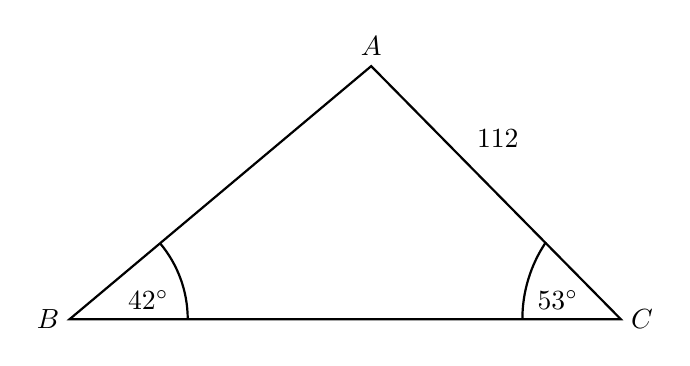
\begin{tikzpicture}[scale=1]
      \draw [thick](40:5)node[above]{$A$}--
      (0,0)node[left]{$B$}--
      (0:7)node[right]{$C$}--cycle;
      \node at (25:6)[below]{$112$};
      \draw [thick, -] (0:1.5) arc [start angle=0, end angle=40, radius=1.5];
      \node at (0:1)[above]{$42^\circ$};
      \draw [thick, -] (0:5.75) arc [start angle=180, end angle=146, radius=1.75];
      \node at (0:6.2)[above]{$53^\circ$};
    \end{tikzpicture}
  \end{flushright}\vspace{2cm}

\newpage
\item Triangle $ABC$ is drawn with $AC=10.5$ cm, $BC=11.0$ cm, and $A\hat{B}C=47^\circ$. \\[0.25cm]
Find $B\hat{A}C$.
  \begin{flushright}
    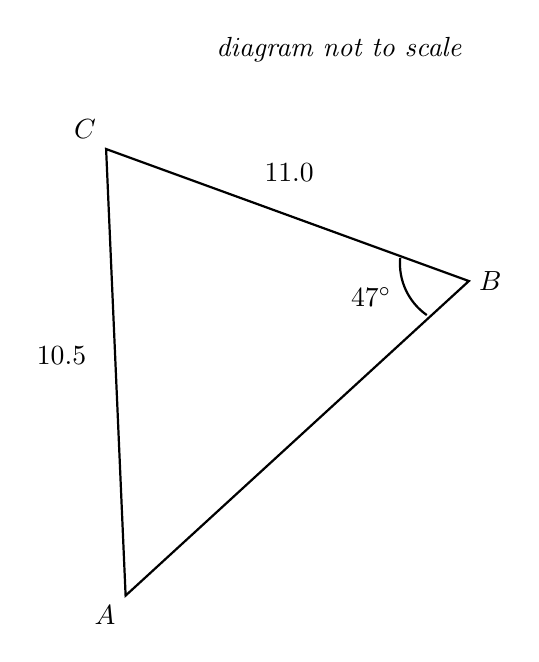
\begin{tikzpicture}[scale=0.8, rotate=20]
      \draw [thick](0:4)node[right]{$B$}--
      (100:4)node[above left]{$C$}--
      (-135:4)node[below left]{$A$}--cycle;
      \node at (55:3.5)[below]{$11.0$};
      \node at (150:2.75)[below]{$10.5$};
      \draw [thick, -] (-5:3.2) arc [start angle=215, end angle=155, radius=1];
      \node at (0:2.35)[above]{$47^\circ$};
      \node at (50:5)[above]{\emph{diagram not to scale}};
    \end{tikzpicture}
  \end{flushright} \vspace{2cm}
  
\item As shown in the diagram, triangle $ABC$ has $A\hat{B}C=31^\circ$, $AB=88$, and $BC=103$. \\[0.25cm]
Find $AC$. \hfill \emph{diagram not to scale}
  \begin{flushright}
    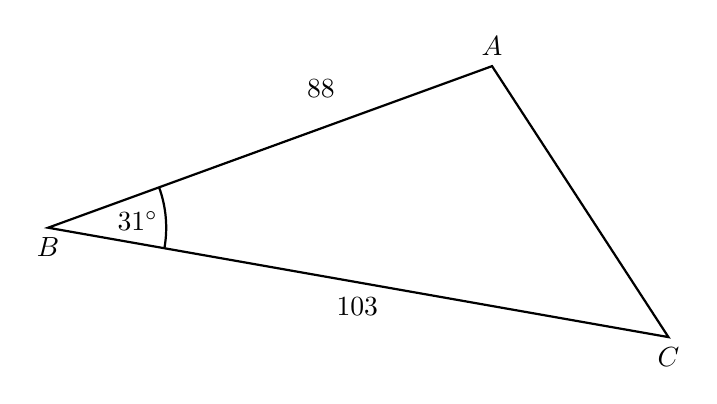
\begin{tikzpicture}[scale=1, rotate=-10]
      \draw [thick](30:6)node[above]{$A$}--
      (0,0)node[below]{$B$}--
      (0:8)node[below]{$C$}--cycle;
      \node at (40:4)[below]{$88$};
      \node at (-1:4)[below]{$103$};
      \draw [thick, -] (0:1.5) arc [start angle=0, end angle=30, radius=1.5];
      \node at (2:1.15)[above]{$31^\circ$};
    \end{tikzpicture}
  \end{flushright}\vspace{3cm}

\newpage
\item The following diagram shows triangle $PQR$. (\emph{not to scale}) \\[0.25cm]
$PQ=55$ meters, $QR=71$ m., and $PR=38$ m. \\[0.25cm]
Find $Q\hat{P}R$.
  \begin{flushright}
    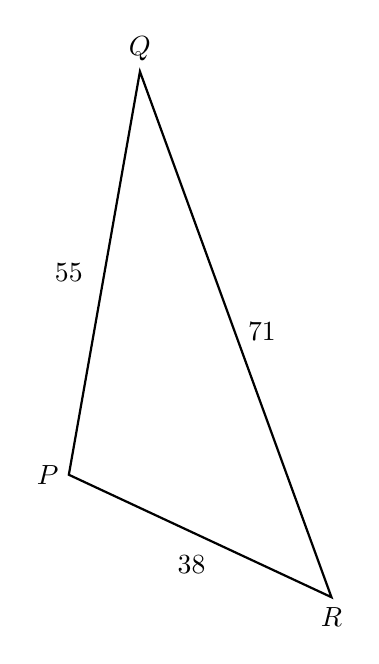
\begin{tikzpicture}[scale=0.8, rotate=20]
      \draw [thick](60:6.5)node[above]{$Q$}--
      (0,0)node[left]{$P$}--
      (-45:4.6)node[below]{$R$}--cycle;
      \node at (70:3.5)[below]{$55$};
      \node at (-50:2.25)[below]{$38$};
      \node at (20:4)[below]{$71$};
    \end{tikzpicture}
  \end{flushright}

\item A ladder that is 6 meters long leans against a wall making an angle to the ground of $73^\circ$, as shown in the diagram.  \hfill (not drawn to scale)
  \begin{multicols}{2}
    \begin{enumerate}
      \item Find the height of the top of the ladder above the ground. \vspace{2cm}
      \item Find the distance of the bottom of the ladder to the base of the wall.
    \end{enumerate} 
    \begin{flushright}
    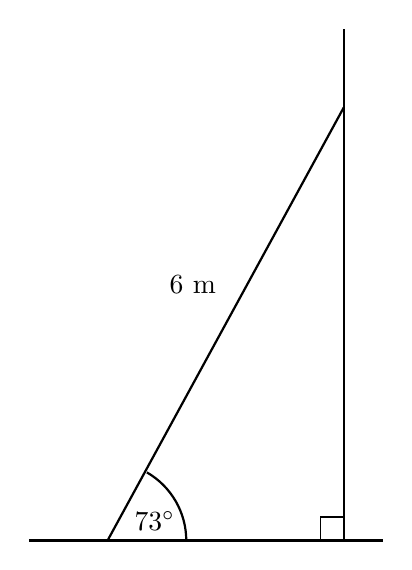
\begin{tikzpicture}[scale=0.5]
      \draw [thick](0,0)--(9,0);
      \draw [thick](8,0)--(8,13);
      \draw [thick](2,0)--(8,11);
      \draw (8,0)++(-0.6,0)--++(0,0.6)--+(0.6,0);
      \node at (5,6.5)[left]{$6$ m};
      \draw [thick, -] (0:4) arc [start angle=0, end angle=60, radius=2];
      \node at (0:3.2)[above]{$73^\circ$};
    \end{tikzpicture}
    \end{flushright}
  \end{multicols}
  \vspace{3cm}

\item The following diagram shows a triangle $ABC$. \hfill (diagram not to scale)\\[0.5cm]
The area of the triangle $ABC$ is 75 $\rm{cm}^2$, $AB=15$ cm, $AC=x$ cm, and $B\hat{A}C = 55^\circ$.
  \begin{multicols}{2}
    \begin{enumerate}
      \item Find $x$.
      \item Find $BC$.
    \end{enumerate}
    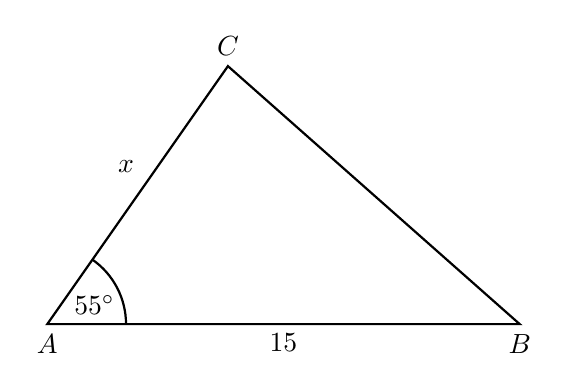
\begin{tikzpicture}[scale=1]
      \draw [thick]
        (0,0)node[below]{$A$}--
        (6,0)node[below]{$B$}--
        (55:4)node[above]{$C$} --cycle;
      \node at (1,2){$x$};
      \node at (3,0)[below]{$15$};
      \draw [thick, -] (1,0) arc [start angle=0, end angle=55, radius=1];
      \node at (0.6,0)[above]{$55^\circ$};
      %\node at (5,0)[below]{$13 \frac{1}{2}$ cm};
    \end{tikzpicture}  
  \end{multicols}
  \vspace{1cm}

\end{enumerate}
\end{document}
